\documentclass{article} % For LaTeX2e
\usepackage{nips15submit_e,times}
\usepackage{hyperref}
\usepackage{url}
\usepackage{lineno}
\usepackage{graphicx}
\usepackage{amsmath}
\usepackage{multicol}
%\usepackage[all]{hypcap} 
\usepackage{listings}
\usepackage{float}
\usepackage{amsfonts}
\usepackage{multicol}
\usepackage{breqn}
\usepackage{bm}
\usepackage{adjustbox}
\setlength{\columnsep}{1cm}
%\linenumbers% Uncomment for line numbers



\title{America's Warzone: Modeling Armed Robberies in Chicago}

\author{
Reuben K. McCreanor\thanks{Department of Statistical Science, Duke University} \\  
\texttt{reuben.mccreanor@duke.edu} \\
\And
Anna K. Yanchenko\footnotemark[1] \\
\texttt{anna.yanchenko@duke.edu} \\
\And 
Lei Qian\footnotemark[1] \\
\texttt{lei.qian@duke.edu} \\
\And
Megan S. Robertson\footnotemark[1] \\
\texttt{megan.robertson@duke.edu} \\ 
}

\hypersetup{
    colorlinks=true,
    linkcolor=blue,
    filecolor=magenta,      
    urlcolor=cyan,
    pdftitle={Sharelatex Example},
    bookmarks=true,
    pdfpagemode=FullScreen,
}


\newcommand{\fix}{\marginpar{FIX}}
\newcommand{\new}{\marginpar{NEW}}

\nipsfinalcopy 

\begin{document}

\maketitle

\section{Introduction}
\label{headings}

\noindent The City of Chicago is frequently listed as one of the most dangerous and crime-ridden cities in the US. President Donald Trump frequently discusses the high-rate of crime in Chicago. According to the Chicago Tribune, there were 4,367 shooting victims in Chicago in 2016. In the same year there were also 785 homicides.\hyperlink{Ref2}{[2]} However, other reports conclude that Chicago should not be called the crime capital?? of America, as Chicago's violence rate is lower than cities like St.  Louis and Detroit. \hyperlink{Ref1}{[1]} The goal of this project was to examine crime in Chicago, specifically armed robberies, from 2012-2016. \newline

\section{Data}
\label{headings}

\noindent The crime data used for this project came from the City of Chicago's website. \footnote{Crimes 2001 to present, \url{https://data.cityofchicago.org/Public-Safety/Crimes-2001-to-present/ijzp-q8t2/data}} The data contained every reported crime in Chicago from 2001 to the present (\autoref{data}). In addition to the type of crime reported (battery, assault, etc.), there was information on the location and time of the crime. The data set was reduced to only consider armed robberies, which we define to be robberies committed with a gun or another type of firearm. 

% \begin{figure}[h]
% \begin{center}
% 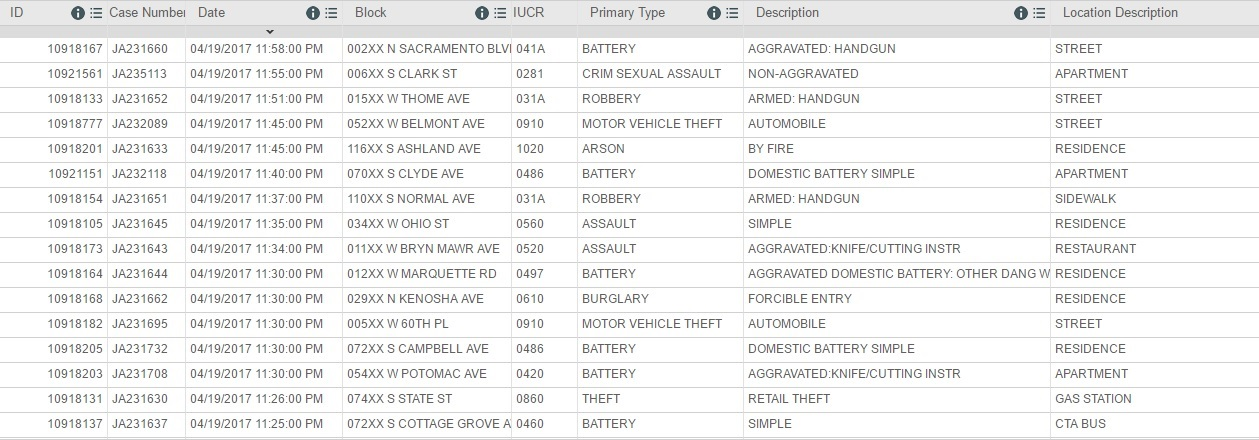
\includegraphics[width=0.8\textwidth,keepaspectratio]{data.jpg}
% \caption{The City of Chicago website provides a data set containing information on crimes committed in the city from 2001 to present day.}
% \label{data}
% \end{center}
% \end{figure}
\begin{table}[h]
\centering
\begin{adjustbox}{width=\textwidth}
\begin{tabular}{ccccccccc}
  \hline
Case Number & Date & Block & Description & Beat & District & Ward & Community Area & Location \\ 
  \hline
HN180091 & 02/16/2007 03:20:00 PM & 012XX W 103RD ST & OTHER WEAPONS VIOLATION & 2232 &  22 &  21 &  73 & (41.706819022, -87.654048084) \\ 
  HN184333 & 02/15/2007 07:00:00 PM & 093XX S WOODLAWN AVE & TELEPHONE THREAT & 413 &   4 &   8 &  47 & (41.725252492, -87.594860893) \\ 
  HN182527 & 02/17/2007 09:00:00 PM & 042XX S COTTAGE GROVE AVE & OTHER VIOLATION & 213 &   2 &   4 &  38 & (41.81741558, -87.606719823) \\ 
  HN183814 & 02/18/2007 10:06:37 PM & 063XX N SHERIDAN RD & TO PROPERTY & 2433 &  24 &  49 &  77 & (41.996866019, -87.655592844) \\ 
  HN182579 & 02/18/2007 12:20:00 AM & 033XX W HURON ST & DOMESTIC BATTERY SIMPLE & 1121 &  11 &  27 &  23 & (41.893682761, -87.710701702) \\ 
  HN182986 & 02/18/2007 10:20:00 AM & 042XX N CENTRAL AVE & OVER \$500 & 1624 &  16 &  38 &  15 & (41.957385814, -87.767141739) \\ 
  HN183716 & 02/18/2007 08:40:00 PM & 037XX S MICHIGAN AVE & DOMESTIC BATTERY SIMPLE & 211 &   2 &   3 &  35 & (41.827167256, -87.623160687) \\ 
  HN184010 & 02/19/2007 02:40:00 AM & 010XX N LAWNDALE AVE & DOMESTIC BATTERY SIMPLE & 1112 &  11 &  27 &  23 & (41.89998654, -87.71890157) \\ 
  HN181071 & 02/17/2007 02:21:00 AM & 051XX S CALUMET AVE & POSS FIREARM/AMMO:NO FOID CARD & 232 &   2 &   3 &  40 & (41.801609105, -87.617736187) \\ 
  HN182079 & 02/17/2007 04:00:00 PM & 034XX W FLOURNOY ST & DOMESTIC BATTERY SIMPLE & 1133 &  11 &  24 &  27 & (41.872709648, -87.711929688) \\ 
  HN184350 & 02/19/2007 12:00:00 AM & 013XX N WOLCOTT AVE & FROM BUILDING & 1424 &  14 &   1 &  24 & (41.905889056, -87.674299261) \\ 
  HN184306 & 02/15/2007 12:01:00 AM & 001XX N PARKSIDE AVE & ILLEGAL USE CASH CARD & 1512 &  15 &  29 &  25 & (41.88301997, -87.766605275) \\ 
  HN183370 & 02/09/2007 10:00:00 AM & 024XX W DEVON AVE & SIMPLE & 2413 &  24 &  50 &   2 & (41.99771689, -87.690448237) \\ 
  HN183500 & 02/18/2007 05:10:00 PM & 070XX S THROOP ST & DOMESTIC BATTERY SIMPLE & 734 &   7 &  17 &  67 & (41.7658997, -87.65656296) \\ 
  HN184055 & 02/19/2007 05:30:00 AM & 005XX W ROSCOE ST & TO RESIDENCE & 2331 &  19 &  44 &   6 & (41.943338611, -87.64332075) \\ 
  HN184352 & 02/19/2007 10:45:00 AM & 003XX N MICHIGAN AVE & FROM BUILDING & 122 &   1 &  42 &  32 & (41.887845852, -87.624560336) \\ 
  HN181018 & 02/17/2007 01:31:00 AM & 056XX S WABASH AVE & TO LAND & 233 &   2 &  20 &  40 & (41.792323044, -87.624025834) \\ 
  HN182857 & 02/18/2007 07:39:41 AM & 014XX W LUNT AVE & FORCIBLE ENTRY & 2431 &  24 &  49 &   1 & (42.009107852, -87.666843608) \\ 
  HN177373 & 02/15/2007 08:44:00 AM & 054XX S CORNELL AVE & TO VEHICLE & 2132 &   2 &   5 &  41 & (41.796263314, -87.585435453) \\ 
  HN183280 & 01/14/2007 12:00:00 PM & 021XX W BIRCHWOOD AVE & DOMESTIC BATTERY SIMPLE & 2424 &  24 &  49 &   1 & (42.017948603, -87.683418074) \\ 
   \hline
\end{tabular}
\end{adjustbox}
\caption{The City of Chicago website provides a data set containing information on crimes committed in the city from 2001 to present day.}
\label{data}
\end{table}



\section{Time Series Analysis}


\noindent The City of Chicago is divided into regions known as sides (\autoref{sides}), where each side is comprised of several neighborhoods. There is a lot of variation in the population (\autoref{population}) and the number of armed robberies per capita (\autoref{counts}) for these sides.  Additionally, some sides are more residential, while others are more commercial.\newline
 
\begin{figure}[h]
\begin{center}

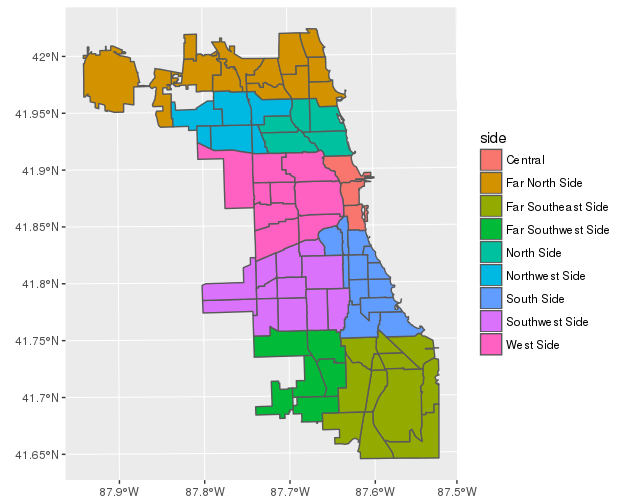
\includegraphics[width=0.8\textwidth,keepaspectratio]{CopyOfside.png}
\caption{The ``sides" of Chicago.  The borders correspond to  the boundaries of the community areas colored by the side.}
\label{sides}
\end{center}
\end{figure}


\begin{figure}[h]
\begin{center}

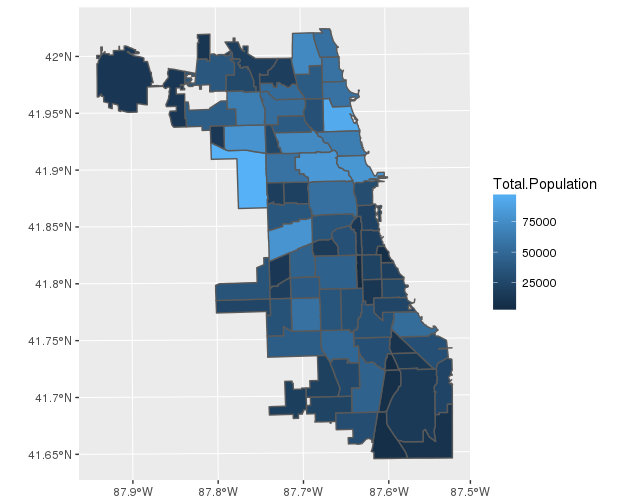
\includegraphics[width=0.8\textwidth,keepaspectratio]{Plots/population.png}
\caption{The population distribution of the  ``sides" of Chicago.  The borders correspond to  the boundaries of the community areas colored by the side.}
\label{population}
\end{center}
\end{figure}

\begin{figure}[h]
\begin{center}

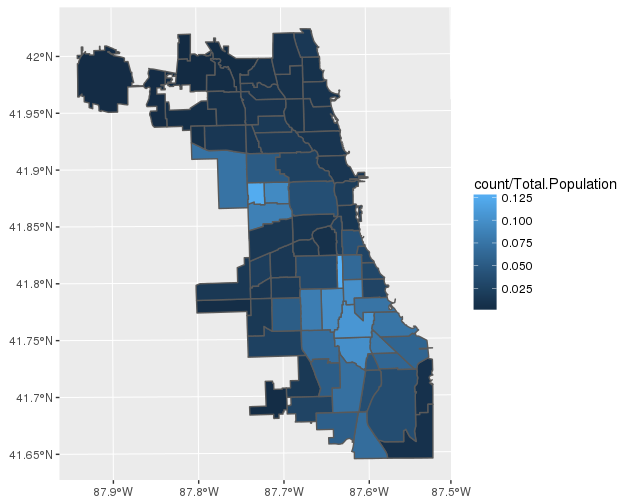
\includegraphics[width=0.8\textwidth,keepaspectratio]{Plots/counts_by_pop.png}
\caption{The number of armed robberies per capita for the ``sides" of Chicago between 2003 and 2016.  The borders correspond to  the boundaries of the community areas colored by the side.}
\label{counts}
\end{center}
\end{figure}

\noindent ARIMA models were fit to predict the counts of monthly armed robberies in each side of the city between 2003 and 2016. In order to determine the type of model, the ACF and PACF plots were examined for the data for each of the sides. For example, if there was structure in the PACF plot beyond one lag, moving average terms were added. The model residuals were also examined to ensure that there was no remaining structure in the residuals. The PACF and ACF plots for the data from the South Side are displayed below. The ACF plot showed evidence of seasonality at lag 12 (i.e. yearly trends). After lag 1, there was no large values for the PACF, so no moving average terms were included in the model. \newline

\break 
\begin{multicols}{2}
\begin{figure}[H]
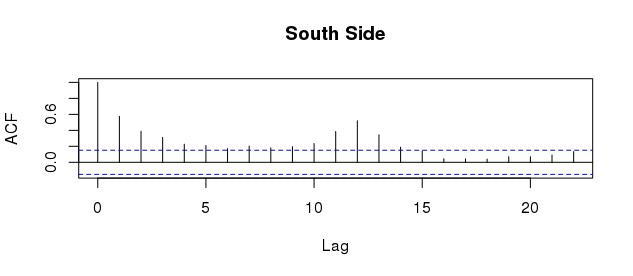
\includegraphics[width=70mm]{Plots/south_ACF.png}
\caption{ACF plot for the number of monthly armed robberies in the South Side of Chicago between 2003 and 2016.}
\end{figure}

\begin{figure}[H]
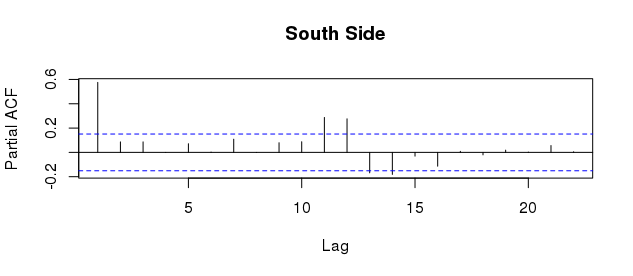
\includegraphics[width=70mm]{Plots/south_PACF.png}
\caption{PACF plot for the number of monthly armed robberies in the South Side of Chicago between 2003 and 2016.}
\end{figure}
\end{multicols}

\noindent Based on the ACF \autoref{south_resid_ACF} and PACF \autoref{south_resid_PACF} plots, an AR(4) model was fit with a seasonal component with period twelve. The residuals plot for this model did not display any remaining structure in the data and the coefficients are in \autoref{south_coef}. 

\begin{multicols}{2}
\begin{figure}[H]
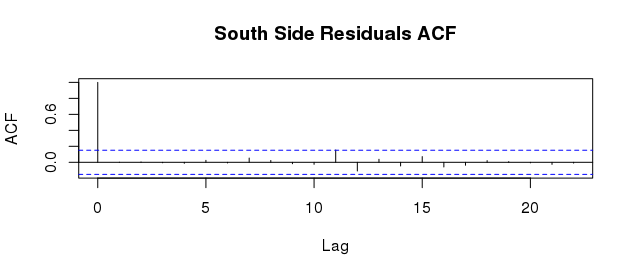
\includegraphics[width=70mm]{Plots/south_resid_ACF.png}
\caption{ACF plot of the residuals of an AR(4) model with a period twelve seasonal component fit to the monthly count of armed robberies for the South Side.}
\label{south_resid_ACF}
\end{figure}

\begin{figure}[H]
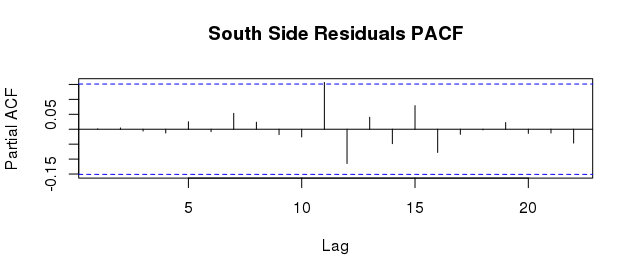
\includegraphics[width=70mm]{Plots/south_resid_PACF.png}
\caption{PACF plot of the residuals of an AR(4) model with a period twelve seasonal component fit to the monthly count of armed robberies for the South Side.}
\end{figure}
\label{south_resid_PACF}
\end{multicols}


\begin{table}[t]
	\label{tab:data}
	\begin{center}
	\begin{tabular}{lccccc}
			\hline
			  & ar1 &    ar2 &    ar3 &    ar4 &   sar1 \\ \hline
			Coefficient & 0.3850 & 0.1328 & 0.0825  & 0.0167 & 0.4784  \\
			Standard Error &   0.0793 & 0.0832&  0.0824 & 0.0771  &0.0708   \\
		\end{tabular}
	\caption{Summary of model fit for the AR(4) with period 12 seasonal component fit to the monthly count of armed robberies for the South Side.}
	\end{center}
\end{table}

\noindent The coefficient estimates for all of the different sides were very similar.  While some sides displayed evidence of higher order autoregressive structure or the addition of moving average terms, as compared to the South Side, all sides had a clear period 12 seasonal component, indicating strong yearly trends for all sides of the city.  The coefficient estimates were positive for the autoregressive terms, indicating that there was a positive correlation between the amount of monthly armed robberies over time.  Plots of the various model fits can be found in \autoref{appendix_regression}.  It is interesting that although the sides of Chicago are quite diverse in terms of population and demographics, as well as the number of monthly armed robberies, the temporal trends for all of the sides are very similar.  Although the count of the monthly armed robberies differs by side of the city, the overall temporal trend is the same across Chicago and has a strong yearly, autoregressive trend.\newline   

\section{Spatial Models}


\subsection{Introduction}

The City of Chicago is comprised of 77 distinct community areas. We predict for counts of armed robbery in each area using a Bayesian Spatial Latent Gaussian Process Poisson Regression Model (BSLGPPR) and a 100 explanatory variables provided by Chicago, \autoref{some table} gathered from a range of years within that of the armed robbery data. We do make the assumption that these variables have not changed much over the next/previous few years and remain applicable. Since we have numerous explanatory variables that range from demographic information to counts of graffiti art, we want to narrow down the number of variables to improve the model's prediction accuracy and interpretability.  A popular frequentist method is the penalized LASSO regression; however, it does not take into account spatial information. Our model, the BSLGPPR, will simulate a LASSO regression while also modeling spatial random effects. 


As the response variable of our data are counts of armed robbery in community areas, we model our observations $\{y_i\}_1^N$, $N = 77$, with a Poisson distribution. 
\begin{equation}
\label{eq:poislhd}
y_i \sim \text{Poisson}(\lambda_i)
\end{equation}
We know that $\lambda_i$ must be positive, which is why we let it equal to the exponential of $\mathbf{X}\boldsymbol{\beta}$. $\boldsymbol{\beta}$ are the coefficients for the explanatory variables and the intercept, which comprises the design matrix$\mathbf{X}$. 
\begin{equation}
\label{eq:lassoLambda}
\log(\boldsymbol{\lambda}) = \mathbf{X}\boldsymbol{\beta}
\end{equation}
\autoref{eq:lassoLambda} is for the LASSO regression, but we will add another variable $\omega_i$ to model random spatial effect in the BSLGPPR model. 
\begin{equation}
\label{eq:spatialLambda}
\log(\boldsymbol{\lambda}) = \mathbf{X}\boldsymbol{\beta} + \boldsymbol{\omega}
\end{equation}


\subsection{The LASSO Model}
\label{lab:LASSO}

Our first model comprises of a simple penalized LASSO regression. Given the positive value of Moran's I, 0.5118399, this model is highly unlikely to outperform one that takes into account the spatial nature of crime. However, we implement this model as a baseline in order to illustrate why the BSLGPPR model performs better.

% As the data is in counts, we use a Poisson penalized regression model under the assumption of Poisson error.
In this model, without the random spatial effect, we do make the assumption that the observations are independent of one another. 

From \autoref{eq:lassoLambda}, it is simple to realize that 
$$ \boldsymbol{\lambda} = e^{\boldsymbol{\beta}'\mathbf{X}}$$.
Given a set of parameters $\boldsymbol{\beta}$, and explanatory variables $\mathbf{X}$, we observe the counts of armed robbery $\mathbf{Y}$ with probability
\begin{equation}
\label{eq:lhd}
p(y_1,..., y_N|\mathbf{x}_1,...,\mathbf{x}_N,\boldsymbol{\beta}) = \prod_{i=1}^{N} \frac{e^{y_i \boldsymbol{\beta}'\mathbf{x}_i}e^{-e^{\boldsymbol{\beta}'\mathbf{x}_i}}}{{y_i}!}
\end{equation}

\autoref{eq:lhd} can be obtained by plugging \autoref{eq:lassoLambda} into the Poisson probability distribution. 

We then want to use the maximum likelihood method to find a set of $\boldsymbol{\beta}$ that will maximize the likelihood, \autoref{eq:lhd} which is the same as maximizing the log-likelihood:
\begin{equation}
\label{eq:loglhd}
l(\boldsymbol{\beta}|\mathbf{X}, \mathbf{Y}) = \sum_{i=1}^N (y_i (\boldsymbol{\beta}' \mathbf{x}_i) - e^{\boldsymbol{\beta}'x_i})
\end{equation}

To implement the penalized LASSO regression, we instead optimize the penalized log-likelihood:
\begin{equation}
\label{eq:penalloglhd}
\min_{\boldsymbol{\beta}} -\frac1N l(\boldsymbol{\beta}|\mathbf{X}, \mathbf{Y})  + \lambda \frac{1}{2} \left((1-\alpha) \sum_{i=1}^N \boldsymbol{\beta}_i^2) +\alpha \sum_{i=1}^N |\boldsymbol{\beta}_i|\right)
\end{equation}
and set $\alpha = 1$.

This method will allow us to obtain more accurate predictions than regular OLS and perform variable selection to prevent overfitting and for interpretability purposes. 






\subsection{The Bayesian Spatial Latent Gaussian Process Poisson Regression Model}

Our second model uses a double exponential or Laplace prior to emulate the LASSO penalized regression model as the distribution sharply peaks at zero; concentrating the probability mass at zero. While this prior will not cause our coefficients to go to zero as in the case of a LASSO--instead behaving more like Ridge regression--we get around this by constructing 95 percent credible intervals around the coefficients and finding the ones that contain zero. 

In our Bayesian model, we use the same data as in \autoref{lab:LASSO} and supplement in spatial data in terms of spatial polygons for the 77 areas. 

For our model, we take \autoref{eq:poislhd} and \autoref{eq:spatialLambda} and further specify by setting: 

$$
\begin{aligned}
\beta_j &\overset{iid}{\sim} \text{Laplace}(0, \eta)\\
\boldsymbol{\omega} &\sim \text{MVN}(\mathbf{0}, \tau(D -\phi W))\\
\tau &\sim \text{Gamma}(2,2)\\
\phi &\sim \text{Unif}(0,0.99)\\
\eta &\sim \text{Unif}(0.001,10)\\
\text{where } \{D:d_\{jj\} &= \text{ total number of neighboring community areas for community area j}| j \in 1...77\} \\  
\text{where } \{W:w_\{jk\} &= \text{whether community area j shares boundaries with community area k}| j,k \in 1...77\}
\end{aligned}
$$

Like before, we say that the armed robbery data can be modeled using a Poisson distribution with $\lambda_i$. We know that $\lambda_i$ must be positive, which is why we let it equal to the exponential of $\mathbf{X}\boldsymbol{\beta} + \omega_i$. $\boldsymbol{\beta}$ are the coefficients for each explanatory variable $\mathbf{X}$ and the intercept. We model the random spatial effect by putting a multivariate gaussian prior on $\omega_i$ and setting the mean to zero,we expect the average effect to be 0, and a correlation matrix $\tau(D -\phi W))$, we believe community areas to be affected by neighboring community areas and the total number of neighboring community areas, which is then scaled by $\tau$ and $\phi$. We set $\tau$ to have a Gamma(2,2) prior because we believe $\tau$ is positive and also heavily concentrated between 0 and 4. $\phi$ has a Unif(0, 0.99) prior to allow for equal probability for any value within the specified range; as we are not biased towards any weight for W. The $\boldsymbol{\beta}$’s are iid Laplace to emulate a penalized LASSO regression. We set $\eta$ to have a Unif(0.001, 10) distribution because we believe that is how concentrated the $\boldsymbol{\beta}$'s will be around the mean, 0; the smaller the $\eta$ the more heavily concentrated at the mean. 



\subsection{Results}

$\boldsymbol{\beta}$ coefficients for the two models can be seen in \autoref{table:betacoef} along with 95\% credible intervals for the BSLGPPR model. To summarize, the LASSO model selects 30 variables whereas BSLGPPR selects 15 variables as seen in \autoref{table:lassoBetaNonZero} and \autoref{table:spatialBetaNonZero}. Predictions are also more accurate as seen in \autoref{fig:spatialplots}; the residuals for the BSLGPPR model are minute compared to that of the LASSO model as the LASSO scale would be approximately 100 times wider than that of the BSLGPPR model. While it seems the predictions in comparison to that of other community areas are similar between the two models, it does not change that BSLGPPR is more accurate. Take a community area such as Austin, predicted to have the highest amount of armed robberies for both models, yet the predicted amount differs by approximately 1000 counts--which is very signficant in this context. 


\begin{table}[h]
\centering
\begin{adjustbox}{width = 0.5\textwidth}
\begin{tabular}{cc}
  \hline
Variable & Lasso \\ 
  \hline
Intercept & 6.5489 \\ 
  Male: 65 and 66 years & -0.3789 \\ 
  Not Hispanic or Latino, Black or African American alone & 0.2773 \\ 
  Assault (Homicide) & 0.2175 \\ 
  Unemployment & -0.2116 \\ 
  Infant Mortality Rate & 0.2030 \\ 
  Vacant Housing Units & 0.1868 \\ 
  Female: 30 to 34 years & 0.1732 \\ 
  Prenatal Care Beginning in First Trimester & -0.1557 \\ 
  Breast cancer in females & 0.1407 \\ 
  N\_Graffiti & 0.1310 \\ 
  Hispanic or Latino & 0.1115 \\ 
  Female: 22 to 24 years & 0.1054 \\ 
  Low Birth Weight & 0.0916 \\ 
  Female: 80 to 84 years & 0.0863 \\ 
  Female: 18 and 19 years & 0.0851 \\ 
  PERCENT AGED 16+ UNEMPLOYED & 0.0847 \\ 
  Tuberculosis & 0.0790 \\ 
  Female: 15 to 17 years & 0.0785 \\ 
  Female: 5 to 9 years & 0.0642 \\ 
  Crowded Housing & -0.0503 \\ 
  Firearm-related & 0.0400 \\ 
  Female: 21 years & 0.0381 \\ 
  Female: 85 years and over & 0.0377 \\ 
  Stroke (Cerebrovascular Disease) & -0.0358 \\ 
  Prostate Cancer in Males & 0.0227 \\ 
  Colorectal Cancer & 0.0124 \\ 
  vacantLots & -0.0080 \\ 
  Not Hispanic or Latino, Asian alone & -0.0045 \\ 
  N\_Aff\_Housing & 0.0006 \\ 
   \hline
\end{tabular}
\end{adjustbox}
\caption{LASSO model's non-zero Beta Coefficients sorted from Most to Least Impact}
\label{table:lassoBetaNonZero}
\end{table}

\begin{table}[h]
\centering
\begin{adjustbox}{width = 0.5\textwidth}
\begin{tabular}{cccc}
  \hline
2.5\% & 97.5\% & Spatial & Variable \\ 
  \hline
6.2136 & 6.2683 & 6.2427 & Intercept \\ 
  -0.8244 & -0.3868 & -0.5845 & Unemployment \\ 
  -0.7821 & -0.1529 & -0.5485 & Male: 45 to 49 years \\ 
  -0.9097 & -0.1008 & -0.4947 & Female: 10 to 14 years \\ 
  0.1699 & 0.5196 & 0.3433 & PERCENT AGED 16+ UNEMPLOYED \\ 
  -0.5641 & -0.0527 & -0.2933 & Male: 65 and 66 years \\ 
  0.1618 & 0.4959 & 0.2893 & Cancer (All Sites) \\ 
  0.0753 & 0.5511 & 0.2888 & Male: 10 to 14 years \\ 
  0.1335 & 0.3318 & 0.2309 & Infant Mortality Rate \\ 
  0.0626 & 0.3982 & 0.2145 & Birth Rate \\ 
  -0.3259 & -0.0923 & -0.2129 & Prenatal Care Beginning in First Trimester \\ 
  0.0968 & 0.3364 & 0.1923 & N\_Graffiti \\ 
  0.0697 & 0.2227 & 0.1423 & Breast cancer in females \\ 
  -0.2459 & -0.0209 & -0.1398 & Not Hispanic or Latino, Asian alone \\ 
  0.0144 & 0.2186 & 0.1282 & Tuberculosis \\ 
  0.0107 & 0.2456 & 0.1021 & Low Birth Weight \\ 
   \hline
\end{tabular}
\end{adjustbox}
\caption{BSLGPPR model's Beta Coefficients that did not contain zero in their 95\% credible interval, sorted from Most to Least Impact}
\label{table:spatialBetaNonZero}
\end{table}

\begin{center}
\begin{figure}[ht]
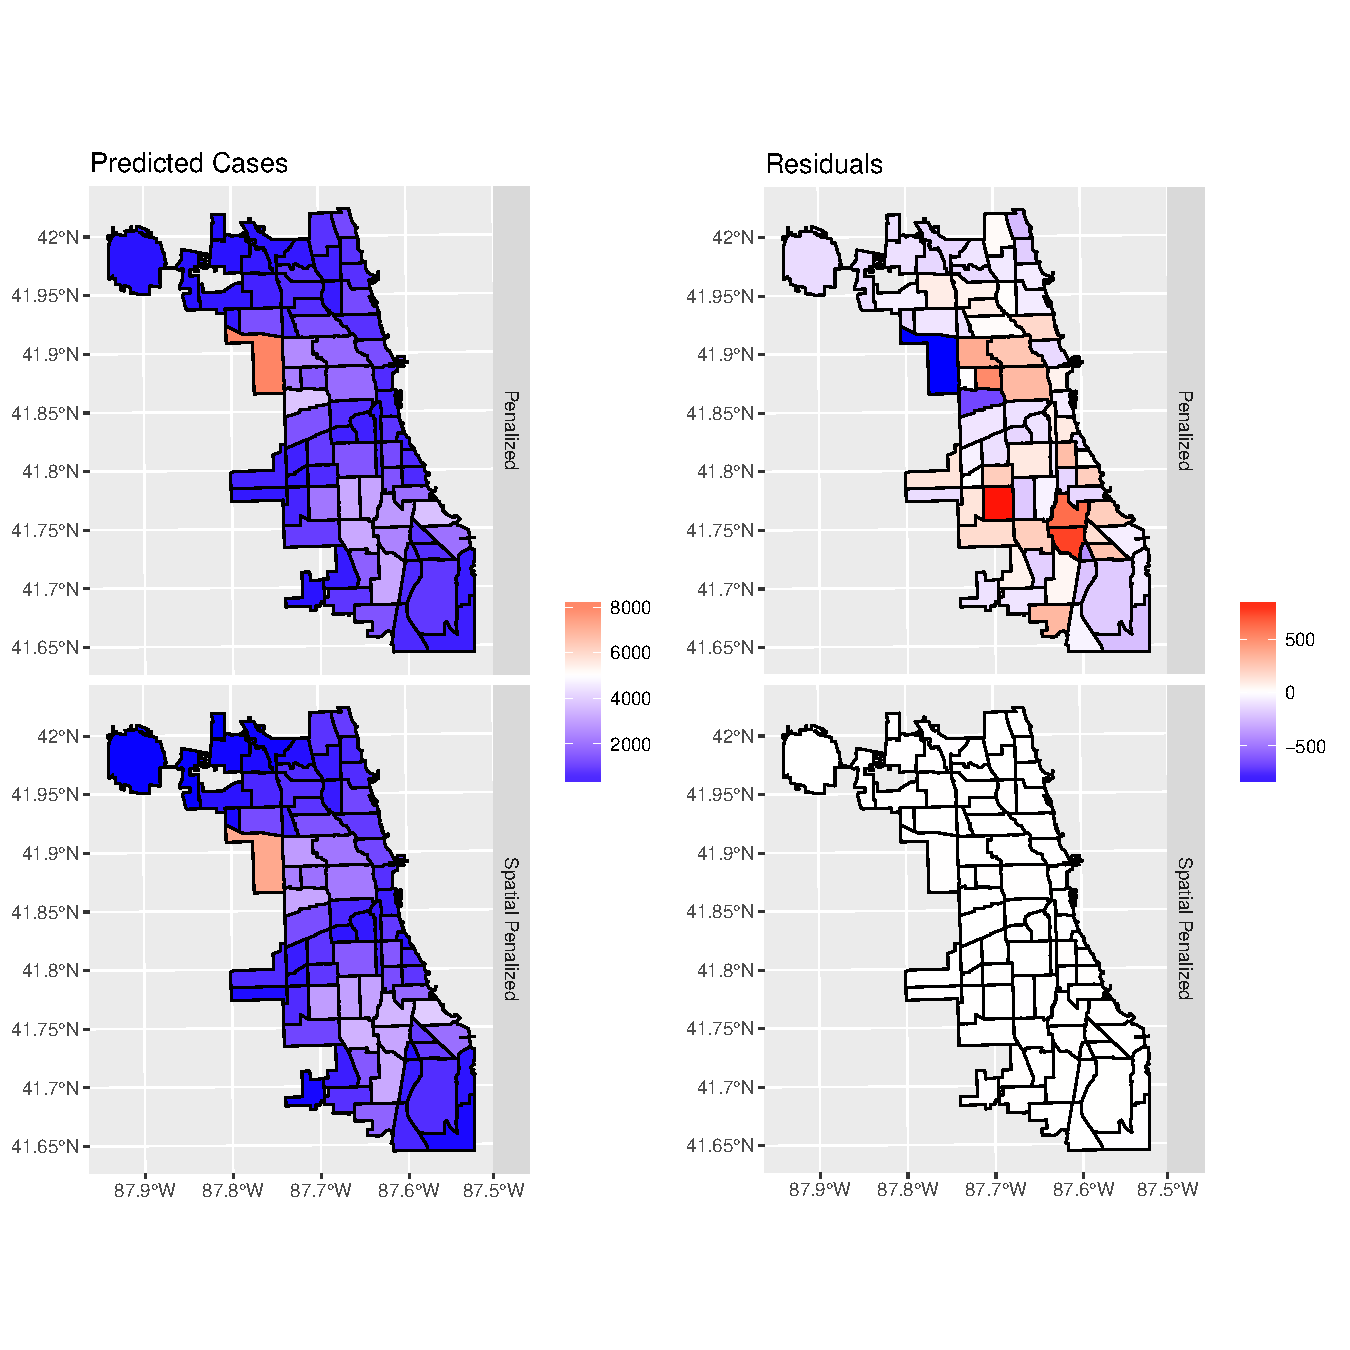
\includegraphics[width = \textwidth]{Plots/results}
\caption{Comparison of Two Model Predictions and Residuals}
\label{fig:spatialplots}
\end{figure}
\end{center}

4 Spatial Models
Intro To Data Spatially - Different Community Areas - Added Variables (100) - What We Want to
Predict - Why Spatial: Moran?s I - How Many Data Points - Why Armed Robbery
LASSO Model
Bayesian Spatial Model
Results + Conclusions - Talk about Austin - Cancer - Residuals Difference - Demographics - Top
Ten Coeffs
- Add Betas in Appendix - Add Reference for Data Sources
- Add Reference for Data Sources 






\newpage


\subsubsection*{References}


\hypertarget{Ref1}{[1]} Papachristos, Andrew V., "48 Years of Crime in Chicago: An Analysis of of Serious Crime Trends from 1965-2013,\url{http://isps.yale.edu/sites/default/files/publication/2013/12/48yearsofcrime_final_ispsworkingpaper023.pdf}, December 2013.

\hypertarget{Ref2}{[2]} Pearson, Rick, "Trump Again Assails Chicago gun violence in speech to Congress", \textit{Chicago Tribune}, \url{http://www.chicagotribune.com/news/local/politics/ct-donald-trump-congress-speech-chicago-met-20170228-story.html}, March 2017.


\clearpage
\newpage

\section{Appendix}
\label{appendix}


\subsection{Time Series Modeling Plots}
\label{appendix_regression}

 
\subsubsection{West Side}
 
\begin{multicols}{2}
 \begin{figure}[H]
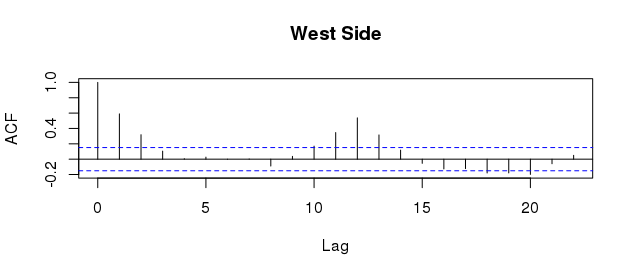
\includegraphics[height=50mm, width=80mm]{Plots/West_ACF.png}
\end{figure}
 
\begin{figure}[H]
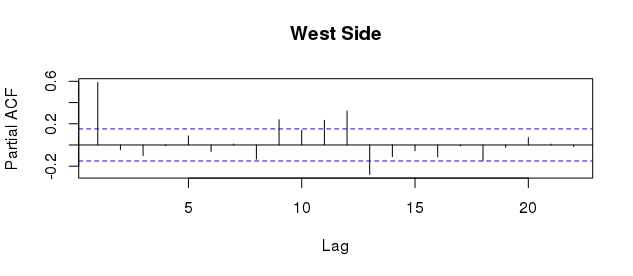
\includegraphics[height=50mm, width=80mm]{Plots/West_PACF.png}
\end{figure}
 
\begin{figure}[H]
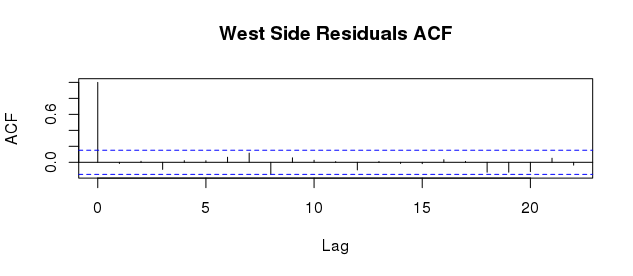
\includegraphics[height=50mm, width=80mm]{Plots/west_resids_ACF.png}
\end{figure}
 
\begin{figure}[H]
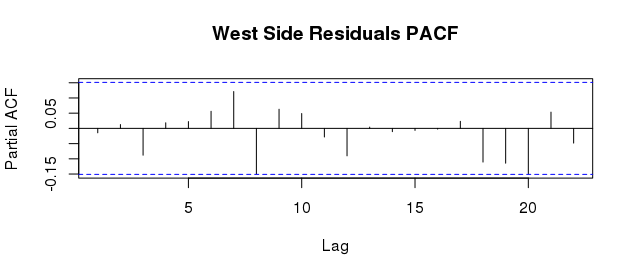
\includegraphics[height=50mm, width=80mm]{Plots/west_resids_PACF.png}
\end{figure}
 \end{multicols}
 
\begin{center}
\begin{figure}[H]
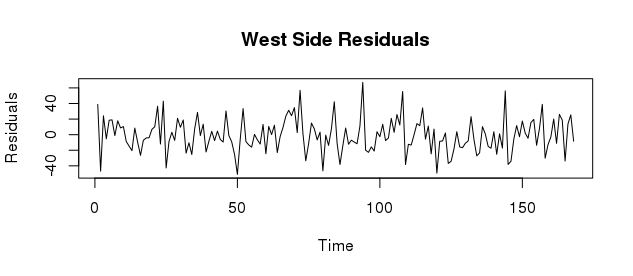
\includegraphics[height=50mm, width=80mm]{Plots/west_resids.png}
\end{figure}
\end{center}
 

 
\subsubsection{Southwest Side}
 
\begin{multicols}{2}
 
\begin{figure}[H]
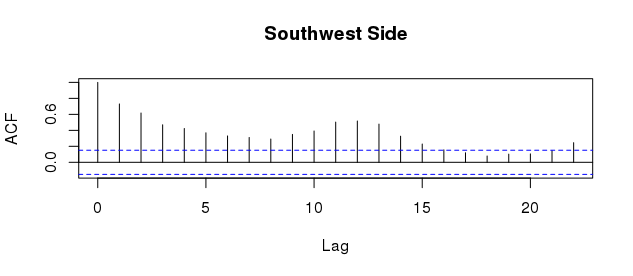
\includegraphics[height=50mm, width=80mm]{Plots/southwest_acf.png}
\end{figure}
 
\begin{figure}[H]
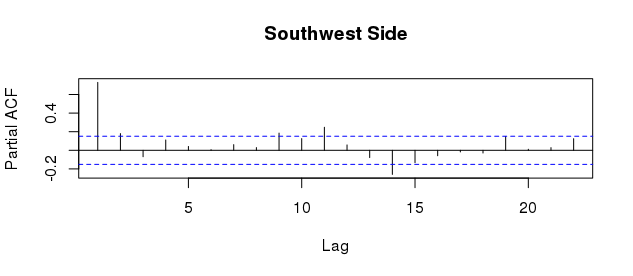
\includegraphics[height=50mm, width=80mm]{Plots/southwest_PACF.png}
\end{figure}
 
\begin{figure}[H]
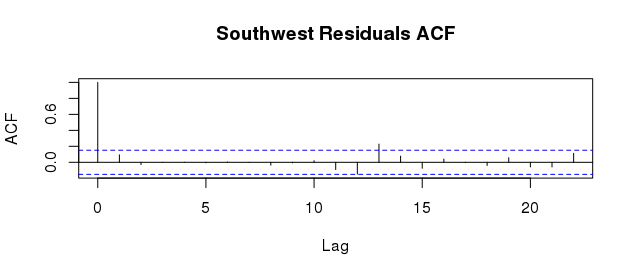
\includegraphics[height=50mm, width=80mm]{Plots/southwest_resid_ACF.png}
\end{figure}
 
\begin{figure}[H]
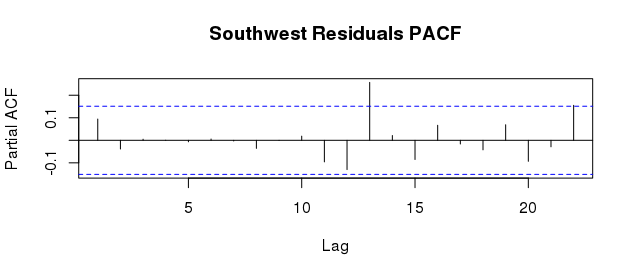
\includegraphics[height=50mm, width=80mm]{Plots/southwest_resid_pacf.png}
\end{figure}
 
\end{multicols}
 
\begin{center}
\begin{figure}[H]
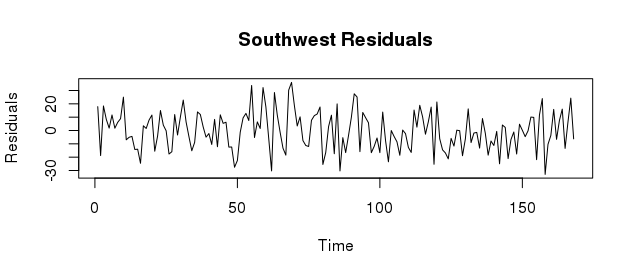
\includegraphics[height=50mm, width=80mm]{Plots/southwest_resid.png}
\end{figure}
\end{center}
 
 
\subsubsection{Southeast Side}
 
\begin{multicols}{2}
 
\begin{figure}[H]
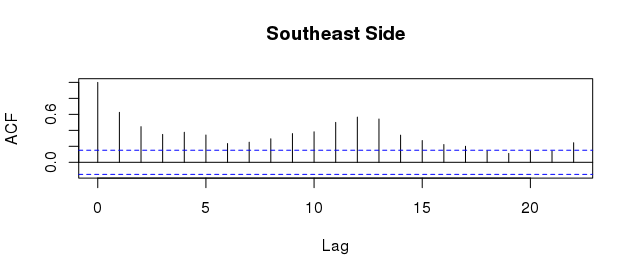
\includegraphics[height=50mm, width=80mm]{Plots/southeast_acf.png}
\end{figure}
 
\begin{figure}[H]
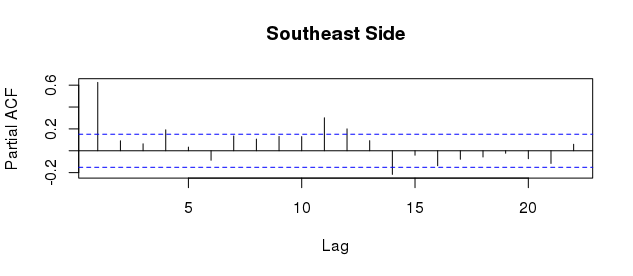
\includegraphics[height=50mm, width=80mm]{Plots/southeast_PACF.png}
\end{figure}
 
\begin{figure}[H]
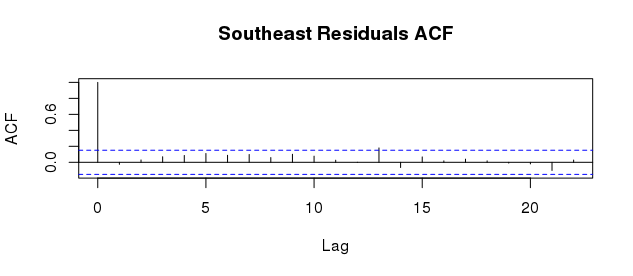
\includegraphics[height=50mm, width=80mm]{Plots/southeast_resid_acf.png}
\end{figure}
 
\begin{figure}[H]
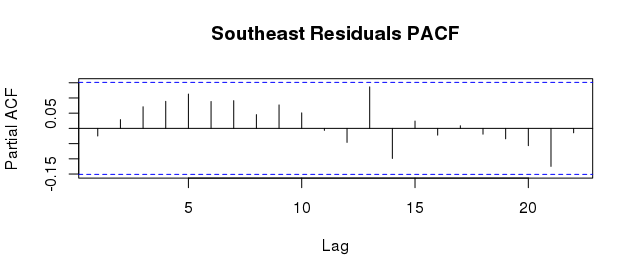
\includegraphics[height=50mm, width=80mm]{Plots/southeast_resid_pacf.png}
\end{figure}
 
\end{multicols}
 
\begin{center}
\begin{figure}[H]
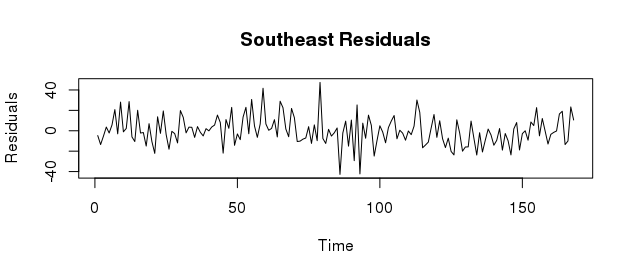
\includegraphics[height=50mm, width=80mm]{Plots/southeast_resid.png}
\end{figure}
\end{center}

 
 
\subsubsection{Northwest Side}
 
\begin{multicols}{2}
 \begin{figure}[H]
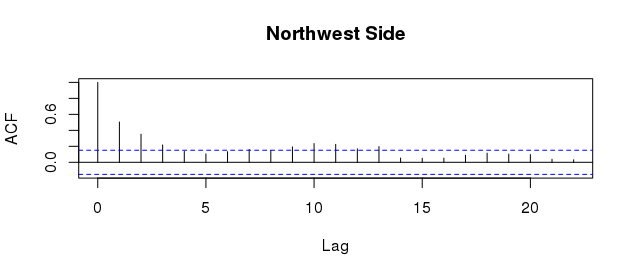
\includegraphics[height=50mm, width=80mm]{Plots/northwest_ACF.png}
\end{figure}
 
\begin{figure}[H]
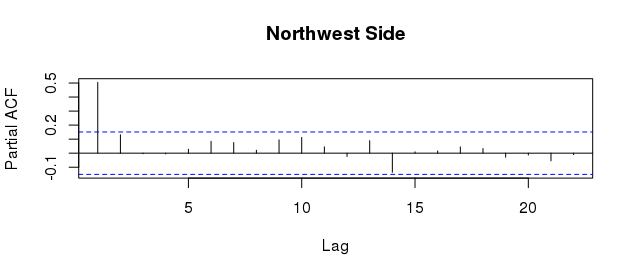
\includegraphics[height=50mm, width=80mm]{Plots/northwest_PACF.png}
\end{figure}
 
\begin{figure}[H]
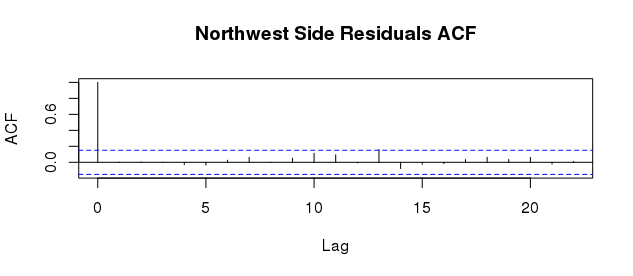
\includegraphics[height=50mm, width=80mm]{Plots/northwest_resid_ACF.png}
\end{figure}
 
\begin{figure}[H]
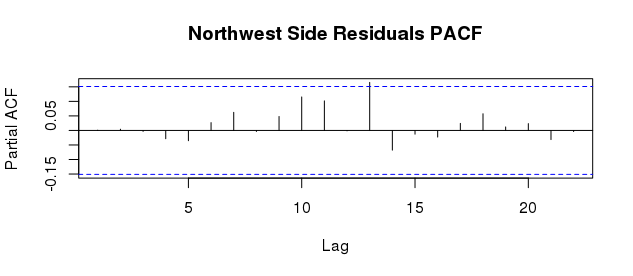
\includegraphics[height=50mm, width=80mm]{Plots/northwest_resid_PACF.png}
\end{figure}
 \end{multicols}
 
\begin{center}
\begin{figure}[H]
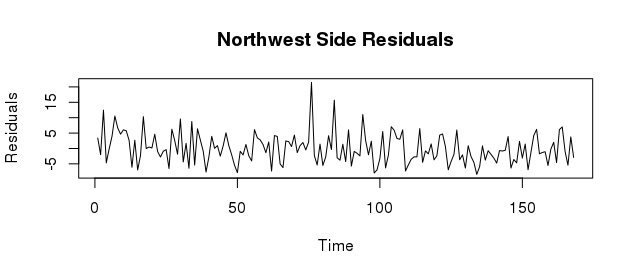
\includegraphics[height=50mm, width=80mm]{Plots/northwest_resids.png}
\end{figure}
\end{center}
 

 
\subsubsection{North Side}
 
\begin{multicols}{2}
 \begin{figure}[H]
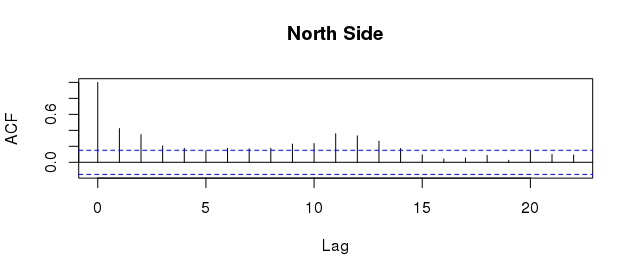
\includegraphics[height=50mm, width=80mm]{Plots/north_ACF.png}
\end{figure}
 
\begin{figure}[H]
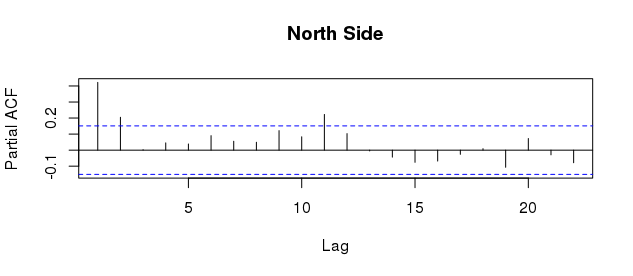
\includegraphics[height=50mm, width=80mm]{Plots/North_PACF.png}
\end{figure}
 
\begin{figure}[H]
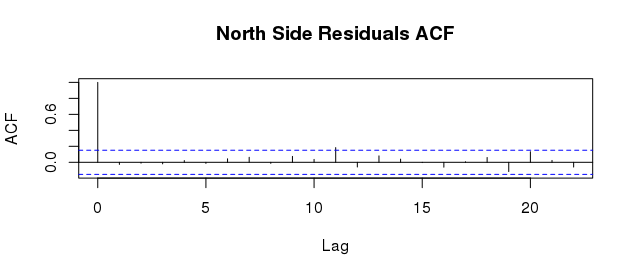
\includegraphics[height=50mm, width=80mm]{Plots/north_resid_ACF.png}
\end{figure}
 
\begin{figure}[H]
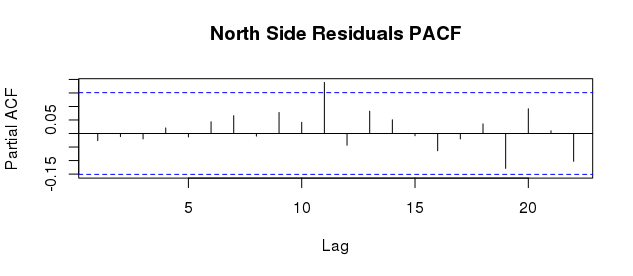
\includegraphics[height=50mm, width=80mm]{Plots/north_resid_PACF.png}
\end{figure}
 \end{multicols}
 
\begin{center}
\begin{figure}[H]
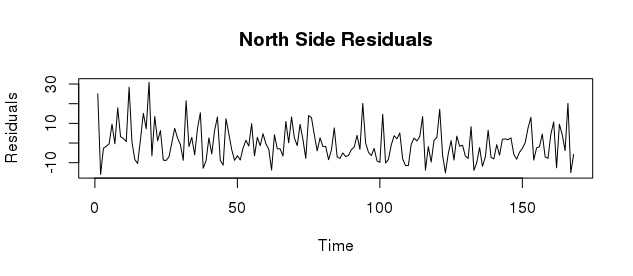
\includegraphics[height=50mm, width=80mm]{Plots/north_residuals.png}
\end{figure}
\end{center}
 

 
\subsubsection{Far Southwest Side}
\begin{multicols}{2} 
\begin{figure}[H]
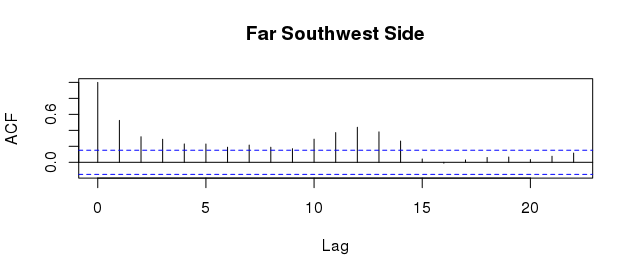
\includegraphics[height=50mm, width=80mm]{Plots/far_southwest_acf.png}
\end{figure}
 
\begin{figure}[H]
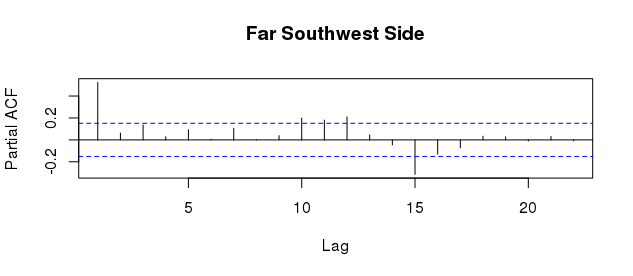
\includegraphics[height=50mm, width=80mm]{Plots/far_southwest_pacf.png}
\end{figure}
 
\begin{figure}[H]
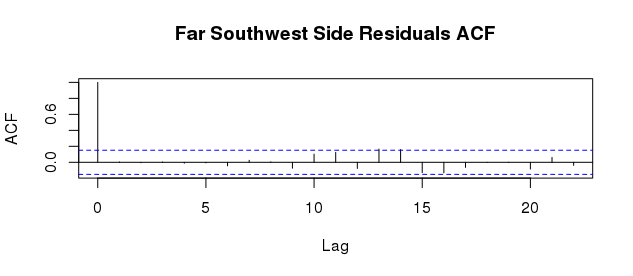
\includegraphics[height=50mm, width=80mm]{Plots/far_southwest_resid_acf.png}
\end{figure}
 
\begin{figure}[H]
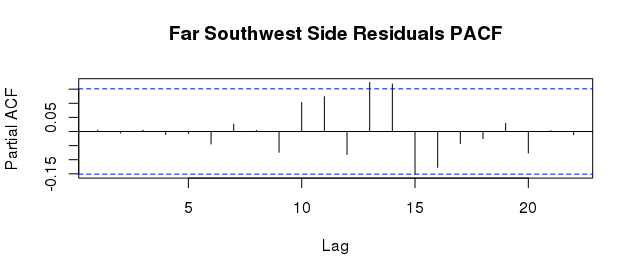
\includegraphics[height=50mm, width=80mm]{Plots/far_southwest_resid_pacf.png}
\end{figure}
 
\end{multicols}
 
\begin{center}
\begin{figure}[H]
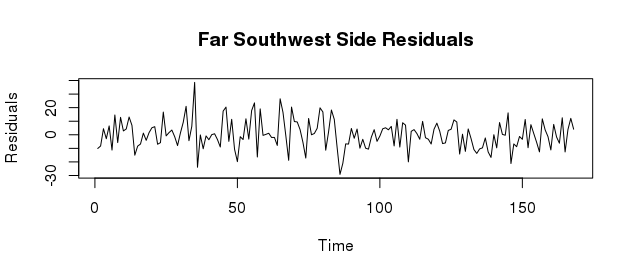
\includegraphics[height=50mm, width=80mm]{Plots/far_southwest_resid.png}
\end{figure}
\end{center}
 

 
\subsubsection{Far North Side}
 
\begin{multicols}{2} 
\begin{figure}[H]
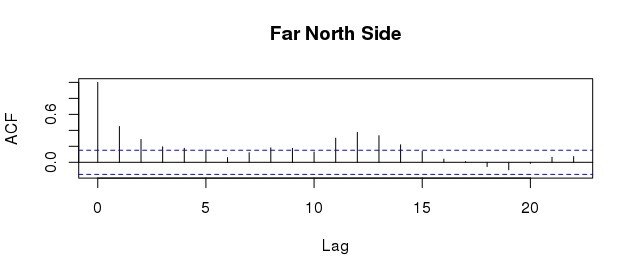
\includegraphics[height=50mm, width=80mm]{Plots/far_north_ACF.png}
\end{figure}
 
\begin{figure}[H]
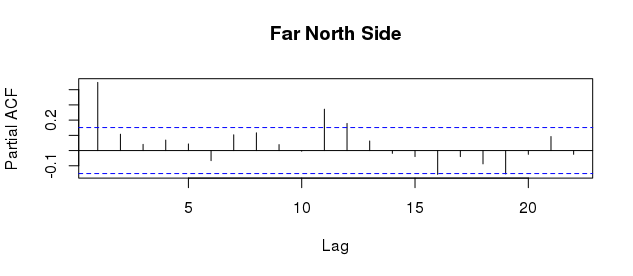
\includegraphics[height=50mm, width=80mm]{Plots/far_north_PACF.png}
\end{figure}
 
\begin{figure}[H]
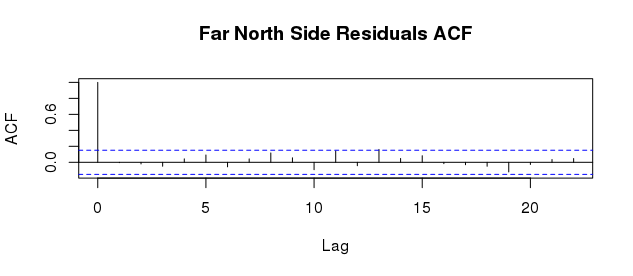
\includegraphics[height=50mm, width=80mm]{Plots/far_north_resids_ACF.png}
\end{figure}
 
\begin{figure}[H]
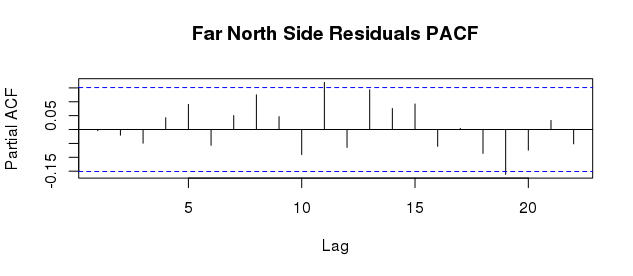
\includegraphics[height=50mm, width=80mm]{Plots/far_north_resids_PACF.png}
\end{figure}
 \end{multicols}
 
\begin{center}
\begin{figure}[H]
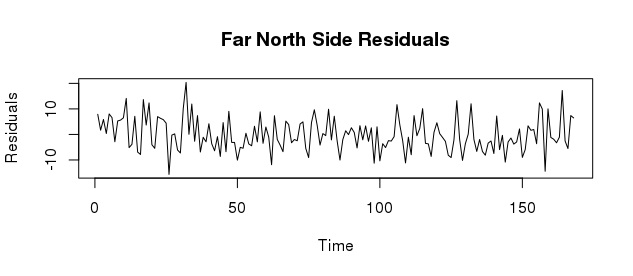
\includegraphics[height=50mm, width=80mm]{Plots/far_north_resids.png}
\end{figure}
 \end{center}
 

 
\subsubsection{Central}
 \begin{multicols}{2}
\begin{figure}[H]
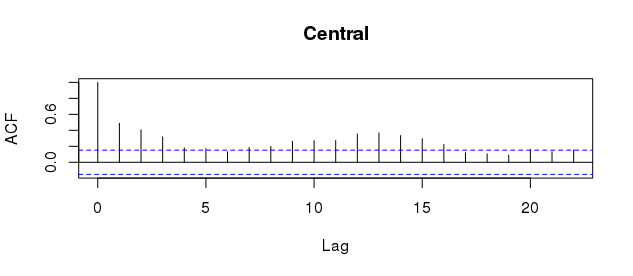
\includegraphics[height=50mm, width=80mm]{Plots/Central_ACF.png}
\end{figure}
 
\begin{figure}[H]
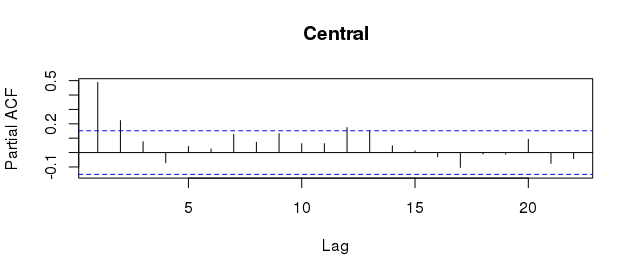
\includegraphics[height=50mm, width=80mm]{Plots/Central_PACF.png}
\end{figure}
 
\begin{figure}[H]
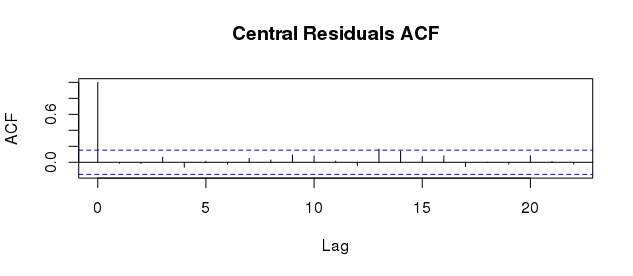
\includegraphics[height=50mm, width=80mm]{Plots/Central_resid_ACF.png}
\end{figure}
 
\begin{figure}[H]
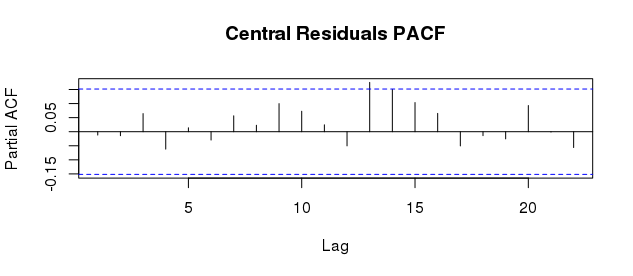
\includegraphics[height=50mm, width=80mm]{Plots/Central_resid_PACF.png}
\end{figure}
 \end{multicols}

\begin{center}
\begin{figure}[H]
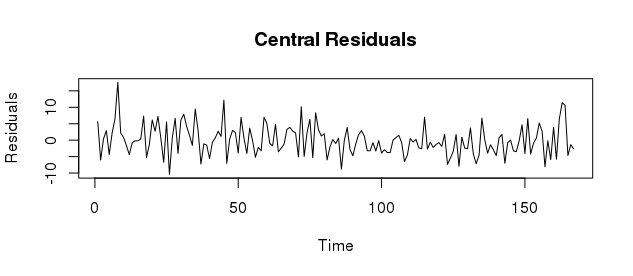
\includegraphics[height=50mm, width=80mm]{Plots/Central_residuals.png}
\end{figure}
\end{center}

\subsection{Spatial Analysis}
\label{appendix_spatial}

\begin{table}[H]
\centering
\begin{adjustbox}{width = \textwidth}
\begin{tabular}{cccccc}
  \hline
Variable & Lasso & 2.5\% & 97.5\% & Spatial & IncludeZero \\ 
  \hline
Intercept & 6.5489 & 6.2136 & 6.2683 & 6.2427 & FALSE \\ 
  KWH Total SQFT & 0.0000 & -0.1712 & 0.4157 & 0.0727 & TRUE \\ 
  THERMS Total SQFT & 0.0000 & -0.2902 & 0.3763 & 0.0674 & TRUE \\ 
  N\_Graffiti & 0.1310 & 0.0968 & 0.3364 & 0.1923 & FALSE \\ 
  Birth Rate & 0.0000 & 0.0626 & 0.3982 & 0.2145 & FALSE \\ 
  General Fertility Rate & 0.0000 & -0.3869 & 0.0174 & -0.1396 & TRUE \\ 
  Low Birth Weight & 0.0916 & 0.0107 & 0.2456 & 0.1021 & FALSE \\ 
  Prenatal Care Beginning in First Trimester & -0.1557 & -0.3259 & -0.0923 & -0.2129 & FALSE \\ 
  Preterm Births & 0.0000 & -0.1675 & 0.0465 & -0.0610 & TRUE \\ 
  Teen Birth Rate & 0.0000 & -0.1547 & 0.1216 & -0.0162 & TRUE \\ 
  Assault (Homicide) & 0.2175 & -0.1223 & 0.3060 & 0.0898 & TRUE \\ 
  Breast cancer in females & 0.1407 & 0.0697 & 0.2227 & 0.1423 & FALSE \\ 
  Cancer (All Sites) & 0.0000 & 0.1618 & 0.4959 & 0.2893 & FALSE \\ 
  Colorectal Cancer & 0.0124 & -0.0272 & 0.1851 & 0.0822 & TRUE \\ 
  Diabetes-related & 0.0000 & -0.1356 & 0.0732 & -0.0433 & TRUE \\ 
  Firearm-related & 0.0400 & -0.0884 & 0.1132 & 0.0265 & TRUE \\ 
  Infant Mortality Rate & 0.2030 & 0.1335 & 0.3318 & 0.2309 & FALSE \\ 
  Lung Cancer & 0.0000 & -0.1050 & 0.1438 & 0.0014 & TRUE \\ 
  Prostate Cancer in Males & 0.0227 & -0.0799 & 0.1437 & 0.0198 & TRUE \\ 
  Stroke (Cerebrovascular Disease) & -0.0358 & -0.1426 & 0.0592 & -0.0379 & TRUE \\ 
  Tuberculosis & 0.0790 & 0.0144 & 0.2186 & 0.1282 & FALSE \\ 
  Below Poverty Level & 0.0000 & -0.0601 & 0.2703 & 0.0843 & TRUE \\ 
  Crowded Housing & -0.0503 & -0.3545 & 0.0036 & -0.1928 & TRUE \\ 
  Dependency & 0.0000 & -0.0464 & 0.2258 & 0.0723 & TRUE \\ 
  No High School Diploma & 0.0000 & -0.1632 & 0.3010 & 0.0759 & TRUE \\ 
  Per Capita Income & 0.0000 & -0.2785 & 0.2422 & -0.0064 & TRUE \\ 
  Unemployment & -0.2116 & -0.8244 & -0.3868 & -0.5845 & FALSE \\ 
  N\_Aff\_Housing & 0.0006 & -0.0934 & 0.0205 & -0.0323 & TRUE \\ 
  PERCENT OF HOUSING CROWDED & 0.0000 & -0.1809 & 0.0931 & -0.0349 & TRUE \\ 
  PERCENT HOUSEHOLDS BELOW POVERTY & 0.0000 & -0.2042 & 0.2440 & -0.0041 & TRUE \\ 
  PERCENT AGED 16+ UNEMPLOYED & 0.0847 & 0.1699 & 0.5196 & 0.3433 & FALSE \\ 
  PERCENT AGED 25+ WITHOUT HIGH SCHOOL DIPLOMA & 0.0000 & -0.2138 & 0.4319 & 0.1477 & TRUE \\ 
  PERCENT AGED UNDER 18 OR OVER 64 & 0.0000 & -0.2190 & 0.2157 & -0.0505 & TRUE \\ 
  PER CAPITA INCOME & 0.0000 & -0.1572 & 0.1933 & 0.0253 & TRUE \\ 
  HARDSHIP INDEX & 0.0000 & -0.1290 & 0.6274 & 0.1752 & TRUE \\ 
  vacantLots & -0.0080 & -0.0200 & 0.0946 & 0.0451 & TRUE \\ 
  Total Population & 0.0000 & -0.0719 & 0.3466 & 0.1129 & TRUE \\ 
  Not Hispanic or Latino, White alone & 0.0000 & -0.3291 & 0.1993 & -0.0750 & TRUE \\ 
  Not Hispanic or Latino, Black or African American alone & 0.2773 & -0.1242 & 0.1845 & 0.0646 & TRUE \\ 
  Not Hispanic or Latino, American Indian and Alaska Native alone & 0.0000 & -0.1491 & 0.2238 & 0.0764 & TRUE \\ 
  Not Hispanic or Latino, Asian alone & -0.0045 & -0.2459 & -0.0209 & -0.1398 & FALSE \\ 
  Not Hispanic or Latino, Native Hawaiian and Other Pacific Islander alone & 0.0000 & -0.0508 & 0.0893 & 0.0065 & TRUE \\ 
  Not Hispanic or Latino, Some Other Race alone & 0.0000 & -0.1073 & 0.3309 & 0.1343 & TRUE \\ 
  Not Hispanic or Latino, Two or More Races & 0.0000 & -0.3185 & 0.3276 & 0.0182 & TRUE \\ 
  Hispanic or Latino & 0.1115 & -0.2077 & 0.1797 & 0.0237 & TRUE \\ 
  Male: Under 5 years old & 0.0000 & -0.1909 & 0.1494 & -0.0237 & TRUE \\ 
  Male: 5 to 9 years & 0.0000 & -0.2622 & 0.0710 & -0.0919 & TRUE \\ 
  Male: 10 to 14 years & 0.0000 & 0.0753 & 0.5511 & 0.2888 & FALSE \\ 
  Male: 15 to 17 years & 0.0000 & -0.3138 & 0.2186 & 0.0197 & TRUE \\ 
  Male: 18 and 19 years & 0.0000 & -0.0289 & 0.7760 & 0.3415 & TRUE \\ 
  Male: 20 years & 0.0000 & -0.0030 & 0.3619 & 0.1537 & TRUE \\ 
  Male: 21 years & 0.0000 & -0.3656 & 0.1339 & -0.0838 & TRUE \\ 
  Male: 22 to 24 years & 0.0000 & -0.1454 & 0.3723 & 0.0717 & TRUE \\ 
  Male: 25 to 29 years & 0.0000 & -0.1612 & 0.4841 & 0.1711 & TRUE \\ 
  Male: 30 to 34 years & 0.0000 & -0.4044 & 0.1591 & -0.0959 & TRUE \\ 
  Male: 35 to 39 years & 0.0000 & -0.4585 & 0.3307 & 0.0278 & TRUE \\ 
  Male: 40 to 44 years & 0.0000 & -0.2925 & 0.2505 & 0.0403 & TRUE \\ 
  Male: 45 to 49 years & 0.0000 & -0.7821 & -0.1529 & -0.5485 & FALSE \\ 
  Male: 50 to 54 years & 0.0000 & -0.2311 & 0.2038 & -0.0092 & TRUE \\ 
  Male: 55 to 59 years & 0.0000 & -0.1085 & 0.5342 & 0.1661 & TRUE \\ 
  Male: 60 and 61 years & 0.0000 & -0.1383 & 0.3300 & 0.0697 & TRUE \\ 
  Male: 62 to 64 years & 0.0000 & -0.4629 & 0.0427 & -0.2165 & TRUE \\ 
  Male: 65 and 66 years & -0.3789 & -0.5641 & -0.0527 & -0.2933 & FALSE \\ 
  Male: 67 to 69 years & 0.0000 & -0.2136 & 0.2511 & 0.0377 & TRUE \\ 
  Male: 70 to 74 years & 0.0000 & -0.4171 & 0.0526 & -0.1750 & TRUE \\ 
  Male: 75 to 79 years & 0.0000 & -0.2765 & 0.1980 & -0.0323 & TRUE \\ 
  Male: 80 to 84 years & 0.0000 & -0.1820 & 0.1216 & -0.0021 & TRUE \\ 
  Male: 85 years and over & 0.0000 & -0.1266 & 0.2376 & 0.0535 & TRUE \\ 
  Female: Under 5 years old & 0.0000 & -0.0854 & 0.3244 & 0.0571 & TRUE \\ 
  Female: 5 to 9 years & 0.0642 & -0.2919 & 0.4038 & 0.0265 & TRUE \\ 
  Female: 10 to 14 years & 0.0000 & -0.9097 & -0.1008 & -0.4947 & FALSE \\ 
  Female: 15 to 17 years & 0.0785 & -0.1623 & 0.2829 & 0.0487 & TRUE \\ 
  Female: 18 and 19 years & 0.0851 & -0.2976 & 0.4667 & 0.0772 & TRUE \\ 
  Female: 20 years & 0.0000 & -0.3636 & 0.1191 & -0.1461 & TRUE \\ 
  Female: 21 years & 0.0381 & -0.2372 & 0.1521 & -0.0438 & TRUE \\ 
  Female: 22 to 24 years & 0.1054 & -0.2446 & 0.1472 & -0.0319 & TRUE \\ 
  Female: 25 to 29 years & 0.0000 & -0.2606 & 0.2080 & -0.0201 & TRUE \\ 
  Female: 30 to 34 years & 0.1732 & -0.5229 & 0.2026 & -0.1613 & TRUE \\ 
  Female: 35 to 39 years & 0.0000 & -0.1611 & 0.4163 & 0.1265 & TRUE \\ 
  Female: 40 to 44 years & 0.0000 & -0.0885 & 0.4475 & 0.1260 & TRUE \\ 
  Female: 45 to 49 years & 0.0000 & -0.0847 & 0.3460 & 0.1258 & TRUE \\ 
  Female: 50 to 54 years & 0.0000 & -0.2909 & 0.1965 & -0.0274 & TRUE \\ 
  Female: 55 to 59 years & 0.0000 & -0.1331 & 0.2360 & 0.0520 & TRUE \\ 
  Female: 60 and 61 years & 0.0000 & -0.1194 & 0.5062 & 0.2276 & TRUE \\ 
  Female: 62 to 64 years & 0.0000 & -0.3584 & 0.1626 & -0.1239 & TRUE \\ 
  Female: 65 and 66 years & 0.0000 & -0.1784 & 0.4086 & 0.1105 & TRUE \\ 
  Female: 67 to 69 years & 0.0000 & -0.2072 & 0.3396 & 0.1342 & TRUE \\ 
  Female: 70 to 74 years & 0.0000 & -0.2815 & 0.2031 & -0.0507 & TRUE \\ 
  Female: 75 to 79 years & 0.0000 & -0.2354 & 0.2365 & -0.0560 & TRUE \\ 
  Female: 80 to 84 years & 0.0863 & -0.1139 & 0.4210 & 0.1324 & TRUE \\ 
  Female: 85 years and over & 0.0377 & -0.1938 & 0.1619 & -0.0117 & TRUE \\ 
  Median Age & 0.0000 & -0.0419 & 0.2316 & 0.0797 & TRUE \\ 
  Total Households & 0.0000 & -0.2695 & 0.3955 & 0.0862 & TRUE \\ 
  Average Household Size & 0.0000 & -0.0545 & 0.2095 & 0.0747 & TRUE \\ 
  Total Housing Units & 0.0000 & -0.0947 & 0.9917 & 0.3907 & TRUE \\ 
  Occupied Housing Units & 0.0000 & -0.4459 & 0.1310 & -0.1418 & TRUE \\ 
  Vacant Housing Units & 0.1868 & -0.3502 & 0.0549 & -0.1469 & TRUE \\ 
  Occupied Housing Units\_\_1 & 0.0000 & -0.2624 & 0.2954 & 0.0121 & TRUE \\ 
  Owned with a mortgage or a loan & 0.0000 & -0.1566 & 0.6600 & 0.2384 & TRUE \\ 
  Owned free and clear & 0.0000 & -0.4927 & 0.1434 & -0.0713 & TRUE \\ 
  Renter occupied & 0.0000 & -0.0892 & 0.5038 & 0.1460 & TRUE \\ 
   \hline
\end{tabular}

\end{adjustbox}
\caption{Beta Coefficients for LASSO and BSLGPPR Models}
\label{table:betacoef}
\end{table}

\end{document}


